%% amssamp1.tex is nearly lidentical to amssamp2.tex, except
%% that amssamp2.tex uses the [twocol] option to produce
%% two-column text. Note that the figures and tables need to be
%% placed in text nearthe first callout, not at the end of the 
%% document. Also note that star form is used for figures
%% and tables.
\documentclass[twocol]{ametsoc}

%%%%%%%%%%%%%%%%%%%%%%%%%%%%%%%%
%%% To be entered only if twocol option is used
\journal{jtech}

%  Please choose a journal abbreviation to use above from the following list:
% 
%   jamc     (Journal of Applied Meteorology and Climatology)
%   jtech     (Journal of Atmospheric and Oceanic Technology)
%   jhm      (Journal of Hydrometeorology)
%   jpo     (Journal of Physical Oceanography)
%   jas      (Journal of Atmospheric Sciences)	
%   jcli      (Journal of Climate)
%   mwr      (Monthly Weather Review)
%   wcas      (Weather, Climate, and Society)
%   waf       (Weather and Forecasting)
%   bams (Bulletin of the American Meteorological Society)
%   ei    (Earth Interactions)

%%%%%%%%%%%%%%%%%%%%%%%%%%%%%%%%
%Citations should be of the form ``author year''  not ``author, year''
\bibpunct{(}{)}{;}{a}{}{,}

\title{Smoothing Noisy GPS Data with Tension}

\authors{Jeffrey J. Early\correspondingauthor{Jeffrey J. Early, NorthWest Research Associates, 
				4118 148th Ave NE, Redmond, WA 98052.} and Adam Sykulski}

\affiliation{NorthWest Research Associates} 

\email{jearly@nwra.com}

\abstract{We develop a technique for smoothing noisy GPS data using B-splines with tension. We show how the tension condition routinely employed in smoothing splines can be restated as a maximum likelihood problem and then how the tension parameter can be chosen based on physical reasoning. The GPS errors appear to be non-Gaussian, so we use a t-distribution in the maximum likelihood.  }

\usepackage{tensor}

\begin{document}

\maketitle

%%%%%%%%%%%%%%%%%%%%%%%%%%%%%%%%%%%%%%%%%%%%%%%%%%%%%%%%%%%%%%%%%%%%%
% MAIN BODY OF PAPER
%%%%%%%%%%%%%%%%%%%%%%%%%%%%%%%%%%%%%%%%%%%%%%%%%%%%%%%%%%%%%%%%%%%%%
\section{Introduction}
Global positioning system receivers (now commonly referred to as `a GPS') are used in literally billions of devices around the the world to track positions. The quality of the position data can be quite good, with accuracies down to a few meters (cite gps.gov), but real world effects (such as atmospheric conditions sky blockages, to quote gps.gov) can significantly increase the errors. Kalman filters are often employed to reduce these errors because they can be run in real time (cite something). Here we consider an alternative approach using smoothing B-splines to control errors for data that has been collected and archived.

The data shown here was collected from from oceanic surface \emph{drifters}, floating buoys with drogues tethered 15-30 meters below the ocean surface, depending on the particular experiment. In the past, these drifters have used Argos positioning system which has significantly poorer temporal coverage and position accuracy (cite elipot), but recently more surface drifters have employed GPS receivers and transmitted their data back through Argos or Iridium satellites. The GPS receiver sits on the surface buoy and collects position data, but because of atmospheric conditions or ocean waves, the receivers are sometimes unable to obtain a position, or when they do, it is highly inaccurately. Thus, despite nominal accuracies of a few meters, it is often the case that some positions are off by more than 1000 meters.

In addition to correcting the position errors, it is also important to interpolate the data to a regular grid. Although the sampling period of a GPS receiver can be fixed, because of missing data and time to to acquire signals, the sampling can be quite irregular. Because many analysis techniques require regular sampling (e.g., a Fourier transform), it is necessary to interpolate the signal onto a regular grid. So the approach taken here is not to simply discard poor data, but also to interpolate the position.

For this particular note we will consider nine surface drifters that were deployed in the Sargasso Sea in the summer of 2011. These particular drifters were part of the LatMix experiment (cite BAMs) and recorded data at approximately 30 minute intervals over the course of a week before being retrieved.

The drifter positions are bivariate time series data given as either projected coordinates $(x_i, y_i)$ or longitude/latitude $(\phi_i, \theta_i$) at times $t_i$. The goal is to create a model of position $(x(t),y(t))$ that is continuous in $t$, and perhaps even continuous a higher derivative---such as velocity or acceleration---that best matches the data given an assumed set of errors. Conceptually this task can be divided into two parts, \emph{interpolating} the data to a continuous time series and \emph{smoothing} the data to remove the noise in the positions.

%%%%%%%%%%%%%%%%%%%%%%
%
\section{Interpolation}
%
%%%%%%%%%%%%%%%%%%%%%%

\begin{figure*}[t]
  \centerline{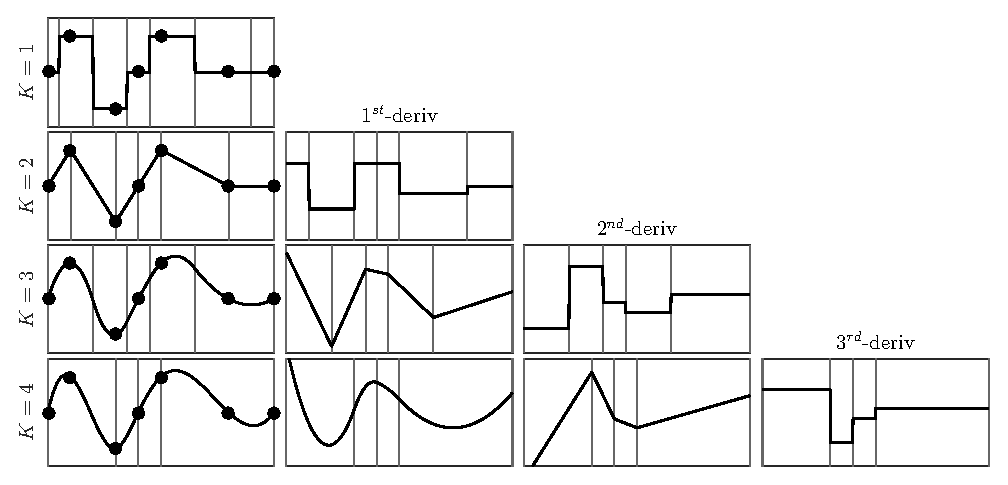
\includegraphics[width=39pc,angle=0]{interpolation}}
  
  \caption{This shows an example of interpolating between 7 data points. The data points are shown as circles, and the interpolated function is shown as a solid black lines. We show four different orders of interpolation $K=1..4$ (rows) and their nonzero derivatives (columns). The thin vertical grey lines are the knot points.}
  \label{interpolation}
\end{figure*}

Assume for the moment that we are given $N$ observations of a particle position $(t_i,x_i)$ with no errors. The simplest possible form of interpolation would be a nearest neighbor method that assigns the position of the particle to the nearest observations in time. The resulting interpolated function $x(t)$ is a polynomial of \emph{order} $K=1$ (piecewise constant), shown in the top row of figure \ref{interpolation}. The next level of sophistication is to assume a constant velocity between any two observations and use that to interpolate positions between observations, second row of figure \ref{interpolation}. This also means that we now have a piecewise constant function $\frac{dx}{dt}$ that represents the velocity of the particle, shown in the second row, second column of figure  \ref{interpolation}. This is a polynomial function of order $K=2$.

It is slightly less obvious how to proceed to a polynomial of order $K=3$. Clearly we want a piecewise constant acceleration (the second derivative), but where to place $\emph{knot points}$ that define the boundaries of the regions  and how to maintain continuity is slightly less clear. The approach taken here is to use B-splines.

%%%%%%%%%%%%%%%%%%%%%%
\subsection{B-Splines}
%%%%%%%%%%%%%%%%%%%%%%

A B-spline (or basis spline) of \emph{order} $K$ (\emph{degree} $S=K-1$) is a piecewise polynomial that maintains nonzero continuity across $S$ knot points. The knot points are a nondecreasing collection of points in time that we will denote with $\tau_i$. The basic theory is well documented in (cite de Boor), but here we will present a reduced version specifically tailored to our needs.

The $m$-th B-spline of order $K=1$ is defined as,
\begin{equation}
X^1_m(t) \equiv \begin{cases}
1      & \text{if $ \tau_m \leq t < \tau_{m+1}$}, \\
0     & \text{otherwise}.
\end{cases}
\end{equation}
This is the rectangle function as shown in the first row, first column of figure \ref{bsplines}. If we are given $P$ knot points, then we can construction $P-1$ B-splines of order $K=1$, although notice that if a knot point is repeated this will result in a splines that is zero everywhere. To represent an interpolating function $x(t)$ for the $N$ observations of a particle position $(t_i,x_i)$ we define $N+1$ knot points as,
\begin{equation}
\tau_m = \begin{cases}
t_1      & \text{$m=1$}, \\
t_{m-1} + \frac{t_{m-1}-t_m}{2}	  & \text{$1<m \leq N$}\\
t_N     & \text{$m>N$}.
\end{cases}
\end{equation}
This will create $N$ independent basis functions that provide support for the region $t_i \leq t \leq t_N$ (provided the last spline is defined to include the last knot point). The interpolating function $x(t)$ is defined as $x(t) \equiv  X^1_m(t) \xi^m$ where the coefficients $\xi^m$ are found by solving $X^1_m(t^i) \xi^m = x^i$. The result of this process is shown in figure \ref{interpolation} for 7 irregularly spaced data points.

All higher order B-splines are defined by recursion,
\begin{equation}
X^K_m(t) \equiv \frac{t - t_m}{t_{m+K-1} - t_m} X^{K-1}_m(t) + \frac{t_{m+K}-t}{t_{m+K} - t_{m+1}} X^{K-1}_{m+1}(t).
\end{equation}
This recursion formula takes two neighboring lower order splines and ramps the left one up over its nonzero domain and ramps the right one down over its nonzero domain. The result of this process is to create splines that span across one additional knot point at each order, and maintain continuity across one more derivatives. Examples are shown in figure \ref{bsplines}.

Any knot points that are repeated $T$ times will result in an a total of $T-1$ splines of order one that are everywhere zero. This has the effect of introducing discontinuities in the derivatives for higher order splines. For our purposes, we will only use this feature to prevent higher order splines from cross the boundaries. For $K=2$ order splines we will use $N+2$ knot points at locations,
\begin{equation}
\tau_m = \begin{cases}
t_1      	& \text{$m \leq 2$}, \\
t_{m-1}	& \text{$2 < m < N$}\\
t_N 		& \text{$m \geq N$}.
\end{cases}
\end{equation}
This creates a knot point at every observation point, but repeats the first and last knot point. This has the effect of terminating the first and last spline at the boundary and creating $N$ second order B-splines, $X^2_m(t)$. Once again the interpolating function $x(t)$ is defined as $x(t) \equiv  X^2_m(t) \xi^m$ where the coefficients $\xi^m$ are found by solving $X^2_m(t^i) \xi^m = x^i$. The second row of figure \ref{interpolation} shows an example.

This process can be continued to higher and higher order B-splines. For splines that are of \emph{even} order, we create $N+K$ knots points with
\begin{equation}
\tau_m^{\text{$K$-even}} = \begin{cases}
t_1      	& \text{$m \leq K$}, \\
t_{m-K/2}	& \text{$K < m < N$}\\
t_N 		& \text{$m \geq N$}
\end{cases}
\label{even-knots}
\end{equation}
and for splines that are \emph{odd} order, we create $N+K$ knot points with,
\begin{equation}
\tau_m^{\text{$K$-odd}} = \begin{cases}
t_1      	& \text{$m \leq K$}, \\
t_{m-\frac{K+1}{2}} + \frac{t_{m-\frac{K+1}{2}}-t_{m-\frac{K+1}{2}+1}}{2}	& \text{$K < m \leq N$}\\
t_N 		& \text{$m > N$}
\end{cases}
\label{odd-knots}
\end{equation}
The knot points are chosen specifically to create $N$ splines for the $N$ data points such that the interpolated function $x(t)$ crosses all $N$ observations $(t_i,x_i)$. Examples are shown in figure \ref{interpolation}.

\begin{figure}
  \centerline{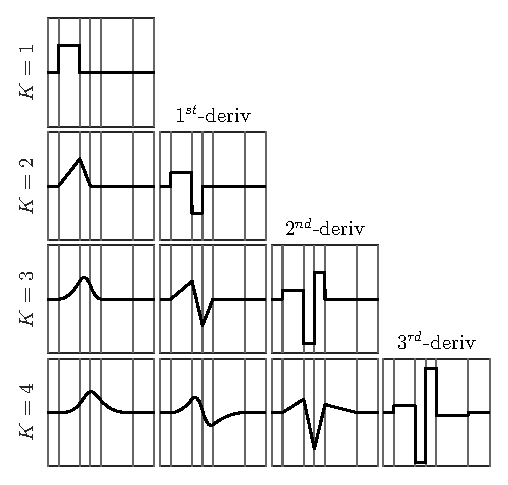
\includegraphics[width=19pc,angle=0]{bsplines}}
  \caption{This shows an example B-spline and its derivatives (columns) for orders $K=1..4$ (rows).}
  \label{bsplines}
\end{figure}

%%%%%%%%%%%%%%%%%%%%%%
%
\section{Maximum Likelihood}
%
%%%%%%%%%%%%%%%%%%%%%%

Using B-splines we now have a mechanism for generating continuous paths given a set of observations, but each observation, $x_i$, differs from the true value, $x(t_i)$, by some noise, $\epsilon_i \equiv x_i - x(t_i)$. The goal now is to find a path $x(t)$ that is not contaminated by the noise.

The approach taken here is to use maximum likelihood. The central idea of maximum likelihood is to ask ``Given a particular path $(x(t),y(t))$, what is the probability that this dataset $(t_i,x_i, y_i)$ could have occurred?'' (cite press et al). The goal is then to find the path that is most likely to have produced that dataset.

Conceptually we have two major pieces that we need to solve this problem:
\begin{enumerate}
\item we need to specify the probability distribution function (PDF) for the errors and
\item we need to specify the form of the path (model).
\end{enumerate}

%%%%%%%%%%%%%%%%%%%%%%
\subsection{Error PDF}
%%%%%%%%%%%%%%%%%%%%%%

The probability function is used to describe the errors in the position, $\epsilon_i$. The canonical example in one-dimension is to assume that the error in our position measurements are Gaussian and therefore the probability of the observed data given the model is,
\begin{equation}
\label{max-gaussian}
P \sim \prod_{i=1}^{N}  \exp \left[ -\frac{1}{2} \left( \frac{x_i - x(t_i)}{\sigma_i} \right)^2 \right] \Delta x
\end{equation}
where $x_i$ represents the observations at time $t_i$ with estimated error of $\sigma_i$.

Maximizing the probability function in equation \ref{max-gaussian} is also the same as minimizing its argument (called the penalty function),
\begin{equation}
\label{least-squares}
\phi =\sum_{i=1}^{N} \left( \frac{x_i - x(t_i)}{\sigma_i} \right)^2 .
\end{equation}
Stated in this way is plain to see that this is the same as asking for the `least-squares' fit of the errors.

%%%%%%%%%%%%%%%%%%%%%%
\subsection{Model}
%%%%%%%%%%%%%%%%%%%%%%

The model used here will be an interpolating B-spline representation of the data at some order $K$ with knot points generated by equations \ref{even-knots} and \ref{odd-knots}. Of course, we've chosen our knot points such that the model intersects each observations and this certainly maximizes equation \ref{max-gaussian} (and minimize equation least-squares) because all the errors are zero, but the resulting distribution of errors (a delta function at zero) doesn't look anything like the assumed Gaussian distribution. Thus, if we want the error distribution that we get out to look like that which we assumed, it also necessary to \emph{constrain} the problem in some way. There are conceptually (at least) two ways of doing this, either 
\begin{enumerate}
\item specify a model with fewer degrees of freedom than data points, or
\item specify an additional \emph{global} constraints on the model in the penalty function.
\end{enumerate}
These two may be equivalent. For example, you may decide the model is a straight line (with two degrees of freedom), or you could set a constraint that that the integral of the second derivative vanish.

We could easily create a model with fewer degrees of freedom than data points by simply removing and rearranging  some of the knot points generated by equations \ref{even-knots} and \ref{odd-knots}. This is certainly worth doing if the data is \emph{oversampled}, where expected distance traversed ($u_{\textrm{rms}}\Delta t$) between observation times ($\Delta t$) is less than the expected error $\sigma_x$. For the cases considered here, we are in an \emph{under-sampled} regime where the drifters have traveled far beyond their the expected error in the time between observations.

The other alternative, and the approach taken here, is to specify a global constraint on the model in the penalty function. In particular, we will use what is known as a smoothing spline.

%%%%%%%%%%%%%%%%%%%%%%
%
\section{Smoothing Spline}
%
%%%%%%%%%%%%%%%%%%%%%%

The smoothing spline augments the penalty function by adding a global constraint on the $m$-th derivative of the resulting function (cite de boor),
\begin{equation}
\label{smoothing-spline}
\phi =  \sum_{i=1}^{N} \left( \frac{x_i - x(t_i)}{\sigma_i} \right) ^2 + \lambda_m \int_{t_1}^{t_N} \left(\frac{d^m x}{dt^m}\right)^2 \, dt.
\end{equation}
If $\lambda_m \rightarrow 0$ then this reduces to the least-squares fit in equation \ref{least-squares}, but if $\lambda_m \rightarrow \infty$ then this forces the model to an $m$-th order polynomial (e.g., when $m=2$, the model will forced to be a straight line because it has no second derivative). 

Assuming a Gaussian distribution in the errors, an appropriate choice for parameter $\lambda$ would reproduce the $\chi^2$-distribution (cite teanby). That is, to say that $\sum \epsilon_i^2/\sigma_i^2 \sim \chi^2_k$, or in the limit of large $N$,  $\frac{1}{N} \sum \epsilon_i^2/\sigma_i^2 \sim 1$.

However, there is a very simple \emph{physical} interpretation for the parameter $\lambda_m$. Consider the case where $m=1$ so that the smoothing spline is a constraint on velocity. When averaged over the integration time, the integral produces the root mean square velocity, $u_{\textrm{rms}}$ so that the penalty function becomes
\begin{equation}
\label{smoothing-spline-velocity}
\phi =  \sum_{i=1}^{N} \left( \frac{x_i - x(t_i)}{\sigma_i} \right) ^2 + \frac{N}{u_{\textrm{rms}}^2 T} \int_{t_1}^{t_N} u^2(t) \, dt.
\end{equation}
where $T\equiv t_N-t_1$. The factor of $N$ in $\lambda_1 =  \frac{N}{u_{\textrm{rms}}^2 T}$ is the scaling for the $\chi^2$ distribution produced by the first term.

The smoothing spline can be restated in terms of maximum likelihood. Assume that in addition to knowing about how the measurement errors are distributed, that we also know how the velocity of underlying physical process is distributed. For example, in geophysical turbulence it has been shown that the velocity probability distribution function is like a two-sided exponential (cite Bracco et al., 2000). Here we will consider the case where the velocity PDF is Gaussian. Stated as maximum likelihood, this means that at \emph{any given instant} (not just the times of observation) we expected the model velocity to look Gaussian. We can discretize the problem by sampling the velocity $Q$ at times $t_q = t_1 + q \Delta t_q$ where $\Delta t_q=\frac{t_N-t_1}{Q-1}$ and $q=0..Q-1$. The maximum likelihood is thus stated as,
\begin{equation}
P \sim \prod^N _{i=1}\exp \left[ -\frac{1}{2} \left( \frac{x_i - x(t_i)}{\sigma_i} \right)^2 \right] \cdot \prod^{Q}_{q=1} \exp \left[  - \frac{1}{2} \left(  \frac{u(t_q)}{\sigma_u} \right)^2 \right] \Delta x.
\end{equation}
Writing this as penalty function (after converting the product of exponentials into exponentials of sums), we have that
\begin{equation}
\phi =  \frac{1}{N} \sum^N _{i=1}\left( \frac{x_i - x(t_i)}{\sigma_i} \right)^2 + \frac{1}{Q} \sum^{Q}_{q=1}  \left(  \frac{u(t_q)}{\sigma_u} \right)^2
\end{equation}
where we've renormalized the error PDF and the velocity PDF to have equal weighting regardless of number of points. Some simple rearranging gives you that,
\begin{equation}
\label{smoothing-spline-pdf}
\phi = \frac{1}{N} \sum^N _{i=1}  \left( \frac{x_i - x(t_i)}{\sigma_i} \right)^2 + \frac{1}{\sigma_u^2 T} \sum^{Q}_{q=1}  u^2(t_q) \Delta t_q.
\end{equation}
Apart from the discretization of the integral, equation \ref{smoothing-spline-velocity} is the same as \ref{smoothing-spline-pdf}. (need to fix the indices for Q).

The implication of this result is that adding tension to the penalty function is equivalent to assuming that one of the higher order derivatives in the model (e.g., acceleration) is Gaussian. This is therefore making an assumption about the \emph{physics} of the model, and not an assumption about the errors. 

%%%%%%%%%%%%%%%%%%%%%%
%
\section{Numerical Implementation}
%
%%%%%%%%%%%%%%%%%%%%%%

The B-splines are generated using the algorithm described in de Boor with knot points determined by equations \ref{even-knots} and \ref{odd-knots}. The matrix $X^i_m$ denotes the $m$-th B-spline at time $t_i$. The first, second and third derivatives of the B-splines are denotes by $V^i_m$, $A^i_m$, $J^i_m$, denoting velocity, acceleration and jerk, respectively.

The covariance matrix describing the measurement errors, $\Sigma\indices{^i_j}$, is taken to be diagonal. In other words, we will assume that the position errors are independent. 

Fully discretized the penalty function is
\begin{equation}
\begin{split}
\phi = \frac{1}{N} \left[ x^k - X\indices{^k_j} \xi^j \right]^{\textrm{T}} \left(\Sigma^{-1}\right)\indices{^k_i} \left[ x^i - X\indices{^i_l} \xi^l \right] \\
+ \frac{1}{Q a_{\textrm{rms}}^2} \left[A\indices{^q_j} \xi^j \right]^{\textrm{T}} \left[ A\indices{^q_l} \xi^l \right].
\end{split}
\end{equation}
To find the coefficients that minimize this function, we take the derivative with respect to $\xi^m$, set it equal to zero, and solve for $\xi^m$,
\begin{equation}
\xi^m = \left[\frac{1}{N} X\indices{_k_j} \left(\Sigma^{-1}\right)\indices{^k_i}  X\indices{^i_m} + \frac{1}{Q a_{\textrm{rms}}^2} {A}\indices{^q_j}{A}\indices{^q_m} \right]^{-1} x_k \left(\Sigma^{-1}\right)\indices{^k_i}   X\indices{^i_j}.
\end{equation}

Let's consider smoothing the acceleration and the jerk because they do not have a well defined mean. There are then two parameters to vary, the assumed standard error of the positions, and the assumed distribution of the acceleration (or jerk). Let's consider two scenarios, one where the position error is large (say 150 meters) and another where the position error is small, say 15 meters, and then choose a tension that gives us the right chi squared distribution. In the first case the resulting error PDF won't look Gaussian, and in the second case the autocorrelation sequence will look bad.

%%%%%%%%%%%%%%%%%%%%%%
\section{Optimal parameters}
%%%%%%%%%%%%%%%%%%%%%%

Fundamentally we have two parameters that we're trying to vary, the error in the position and the rms acceleration. The chi squared statistics mentioned earlier is just part of the idea of trying to find a parameter that forces the expected error PDF to match the PDF that we get out. Of course, we might also try to match the acceleration PDF as well. So the question is then which do we match, the error PDF, the acceleration PDF, or both?

The answer is somewhat philosophical. If the practitioner is highly certain that the errors follow a particular PDF, then it might be advisable to match the error PDFs. On the other hand, perhaps the measurement errors aren't well understood, but the underlying physical process is fairly well understood. In this case you might want to match the more physical metric, the acceleration PDF in this example. This 


But, we're trying to match both of these distributions. So on some level we'd want both to to do well. So we should maximize the joint pdf.


%\begin{acknowledgment} 
%Start acknowledgments here.
%\end{acknowledgment}
%
%% Use appendix}[A], {appendix}[B], etc. etc. in place of appendix if you have multiple appendixes.
%\ifthenelse{\boolean{dc}}
%{}
%{\clearpage}
%\begin{appendix}
%\section*{\begin{center}Appendix Title Is Entered Here (Primary heading)\end{center}}
%\subsection{First appendix secondary heading}
%
%\subsection{Second appendix secondary heading}
%
%\subsubsection{First appendix tertiary heading}
%
%\subsubsection{Second appendix tertiary heading}
%
%\paragraph{First appendix quaternary heading}
%
%\paragraph{Second appendix quaternary heading}
%
%\end{appendix}
%
%% Create a bibliography directory and place your .bib file there.
%% -REMOVE ALL DIRECTORY PATHS TO REFERENCE FILES BEFORE SUBMITTING TO THE AMS FOR PEER REVIEW
%\ifthenelse{\boolean{dc}}
%{}
%{\clearpage}
%\bibliographystyle{ametsoc}
%\bibliography{references}
%
%%%%%%%%%%%%%%%%%%%%%%%%%%%%%%%%%%%%%%%%%%%%%%%%%%%%%%%%%%%%%%%%%%%%%%
%% FIGURES-REMOVE ALL DIRECTORY PATHS TO FIGURE FILES BEFORE SUBMITTING TO THE AMS FOR PEER REVIEW
%%%%%%%%%%%%%%%%%%%%%%%%%%%%%%%%%%%%%%%%%%%%%%%%%%%%%%%%%%%%%%%%%%%%%%
%\begin{figure}[t]
%  \noindent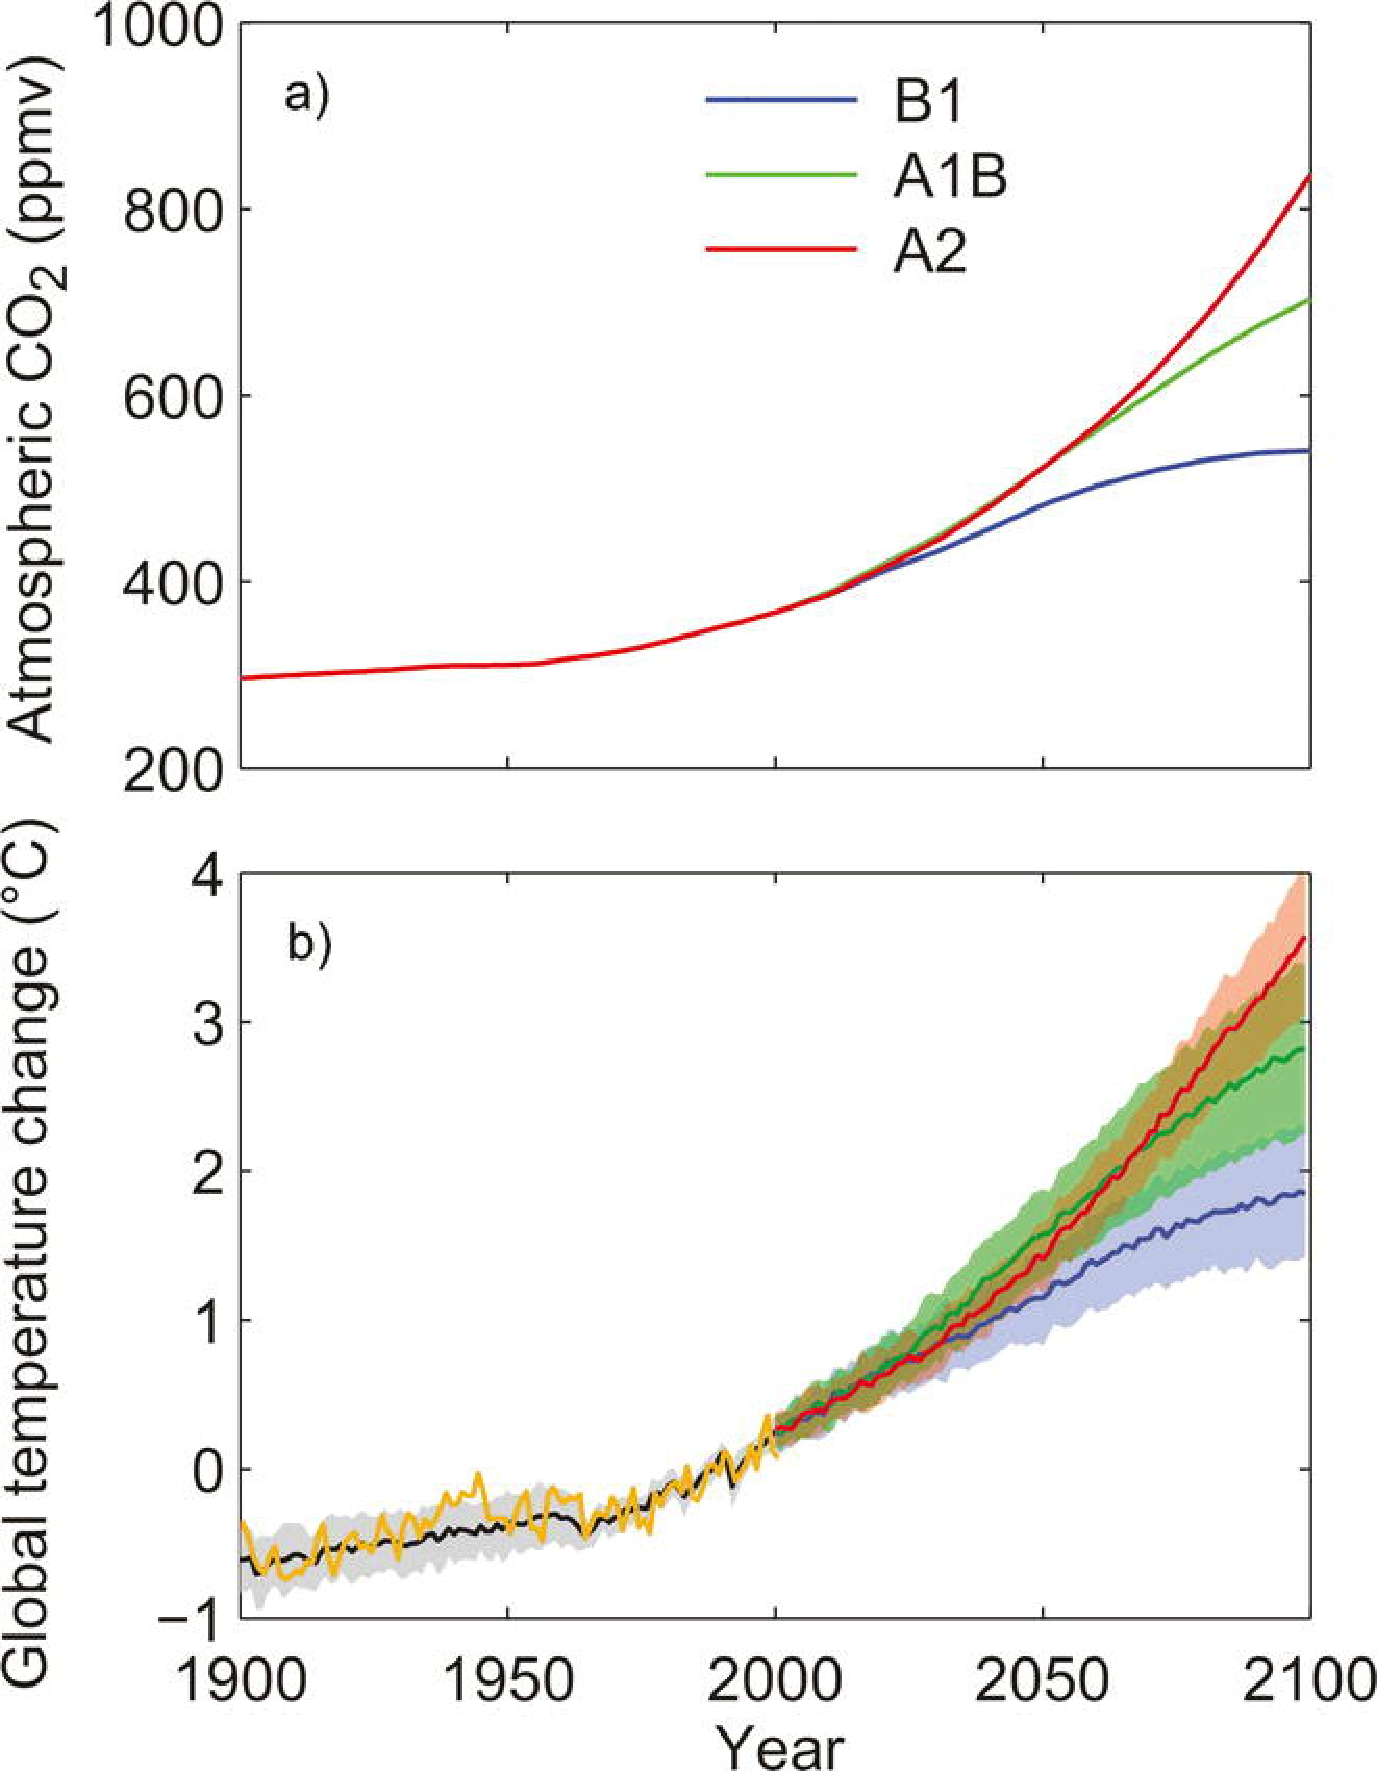
\includegraphics[width=19pc,angle=0]{figure01.pdf}\\
%  \caption{Enter the caption for your figure here.  Repeat as
%  necessary for each of your figures. Figure from \protect\cite{Knutti2008}.}\label{f1}
%\end{figure}
%%%%%%%%%%%%%%%%%%%%%%%%%%%%%%%%%%%%%%%%%%%%%%%%%%%%%%%%%%%%%%%%%%%%%%
%% TABLES
%%%%%%%%%%%%%%%%%%%%%%%%%%%%%%%%%%%%%%%%%%%%%%%%%%%%%%%%%%%%%%%%%%%%%%
%\begin{table}[t]
%\caption{This is a sample table caption and table layout.  Enter as many tables as
%  necessary at the end of your manuscript. Table from Lorenz (1963).}\label{t1}
%\begin{center}
%\begin{tabular}{ccccrrcrc}
%\hline\hline
%$N$ & $X$ & $Y$ & $Z$\\
%\hline
% 0000 & 0000 & 0010 & 0000 \\
% 0005 & 0004 & 0012 & 0000 \\
% 0010 & 0009 & 0020 & 0000 \\
% 0015 & 0016 & 0036 & 0002 \\
% 0020 & 0030 & 0066 & 0007 \\
% 0025 & 0054 & 0115 & 0024 \\
%\hline
%\end{tabular}
%\end{center}
%\end{table}
%
\end{document}